\documentclass{article}
\usepackage{tikz}
\usepackage{amsmath}

\begin{document}

\begin{figure}[h]
    \centering
    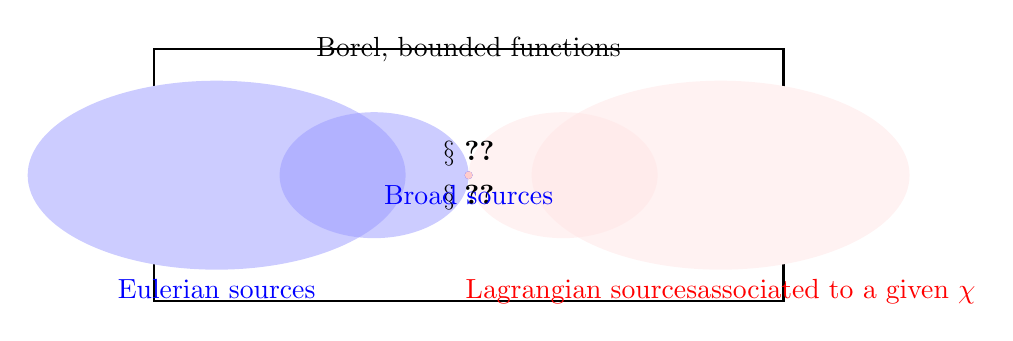
\begin{tikzpicture}[scale=0.8]
        % Draw the rectangle
        \draw[thick] (-5,-2) rectangle (5,2);
        
        % Draw the blue ellipse (Eulerian sources)
        \fill[blue!20] (-4,0) ellipse (3 and 1.5);
        \node at (-4, -1.5) [below] {\textcolor{blue}{Eulerian sources}};
        
        % Draw the pink ellipse (Lagrangian sources associated to a given $\chi$)
        \fill[pink!20] (4,0) ellipse (3 and 1.5);
        \node at (4, -1.5) [below] {\textcolor{red}{Lagrangian sources \\ associated to a given $\chi$}};
        
        % Draw the intersection area
        \fill[blue!40, opacity=0.5] (-1.5,0) ellipse (1.5 and 1);
        \fill[pink!40, opacity=0.5] (1.5,0) ellipse (1.5 and 1);
        
        % Draw the intersection area with labels
        \node at (0, 0) [circle, fill=blue!80, inner sep=1pt] {};
        \node at (0, 0) [circle, fill=pink!80, inner sep=1pt] {};
        \node at (0, 0) [above] {$\S$ \ref{sec:lagrangian}};
        \node at (0, 0) [below] {$\S$ \ref{sec:lagrangian}};
        
        % Draw the intersection area with label
        \node at (0, 0) [below] {\textcolor{blue}{Broad sources}};
        
        % Draw the title
        \node at (0, 2) {Borel, bounded functions};
    \end{tikzpicture}
    \caption{We picture relations among the sources that we determine for a fixed continuous solution of the balance law~\eqref{EE} under the non-degeneracy Assumption~\eqref{ass:h}. When the Lagrangian source is continuous, it is `the' source term in all the formulations.}
    \label{fig:venn_diagram}
\end{figure}

\end{document}